\documentclass[10pt]{article}

\usepackage[T1]{fontenc}
\usepackage[utf8]{inputenc}
\usepackage[french,english]{babel}

\usepackage{graphicx}
\usepackage{textcomp}
\usepackage{float}

\usepackage[export]{adjustbox}

\title{IoT Project:\\Smart House}
\author{Fran\c{c}ois \bsc{Bidet}}
\date{\today}

\begin{document}

\maketitle

\section{Presentation}

My project consists in the simulation of a smart house.

Some sensors are in the house and send data to a server, in or out the house. It can be a computer with a specific software or a specific device as for thermostats fixed on a wall. Those sensors can be temperature sensors, lumen sensors, gas sensors, et caetera.

Some actuators are in the house and receive commands from the server. They can be heaters, lights, electric shutters, windows, et caetera.

For the project, I have used:
\begin{itemize}
\item humiture sensor
\item lumen sensor
\item button
\item dual color led (for heater and air-conditioner representation)
\item RGB led
\end{itemize}

\section{Behavior}

The raspberry plays the role of gateway.
It sends sensors data second to the server.

A computer plays the role of the server. It receives sensors data and it sends commands to the actuators via the raspberry every 5 seconds.

The delays of the sender and receiver are arbitrary fixed. For a real implementation, we need to configure those delays: we need a faster control of lumen than of the temperature.

\subsection{Temperature management}

The server can fixe a reference temperature. When it receives temperature data, it compares to the reference:
\begin{itemize}
  \item if the temperature is lower than the reference, it sends command to turn on the heaters.
  \item if the temperature is higher than the reference, it sends command to turn on the air-conditioner (cooler).
  \item else it sends command to turn off both.
\end{itemize}

When the rapsberry receives command:
\begin{itemize}
\item if it is to turn on the heaters, it fixes the color of the dual-color led to red.
\item if it is to turn on the air-conditioner, it fixes the color of the dual-color led to green.
\item else it turns off the dual-color led.
\end{itemize}

An hysteresis is implemented in the server program but due to the temperature sensor precision (I got entire values like 20.0°C and never 20.3°C), this behavior does not appear.

\begin{figure}[H]
  \centering
  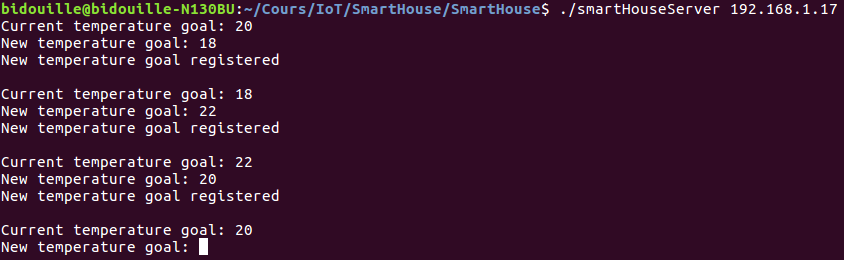
\includegraphics[width=\textwidth]{../imgs/serverInterface.png}
  \caption{\label{serverInterface}Server interface to control the reference temperature}
\end{figure}

\begin{figure}[H]
  \centering
  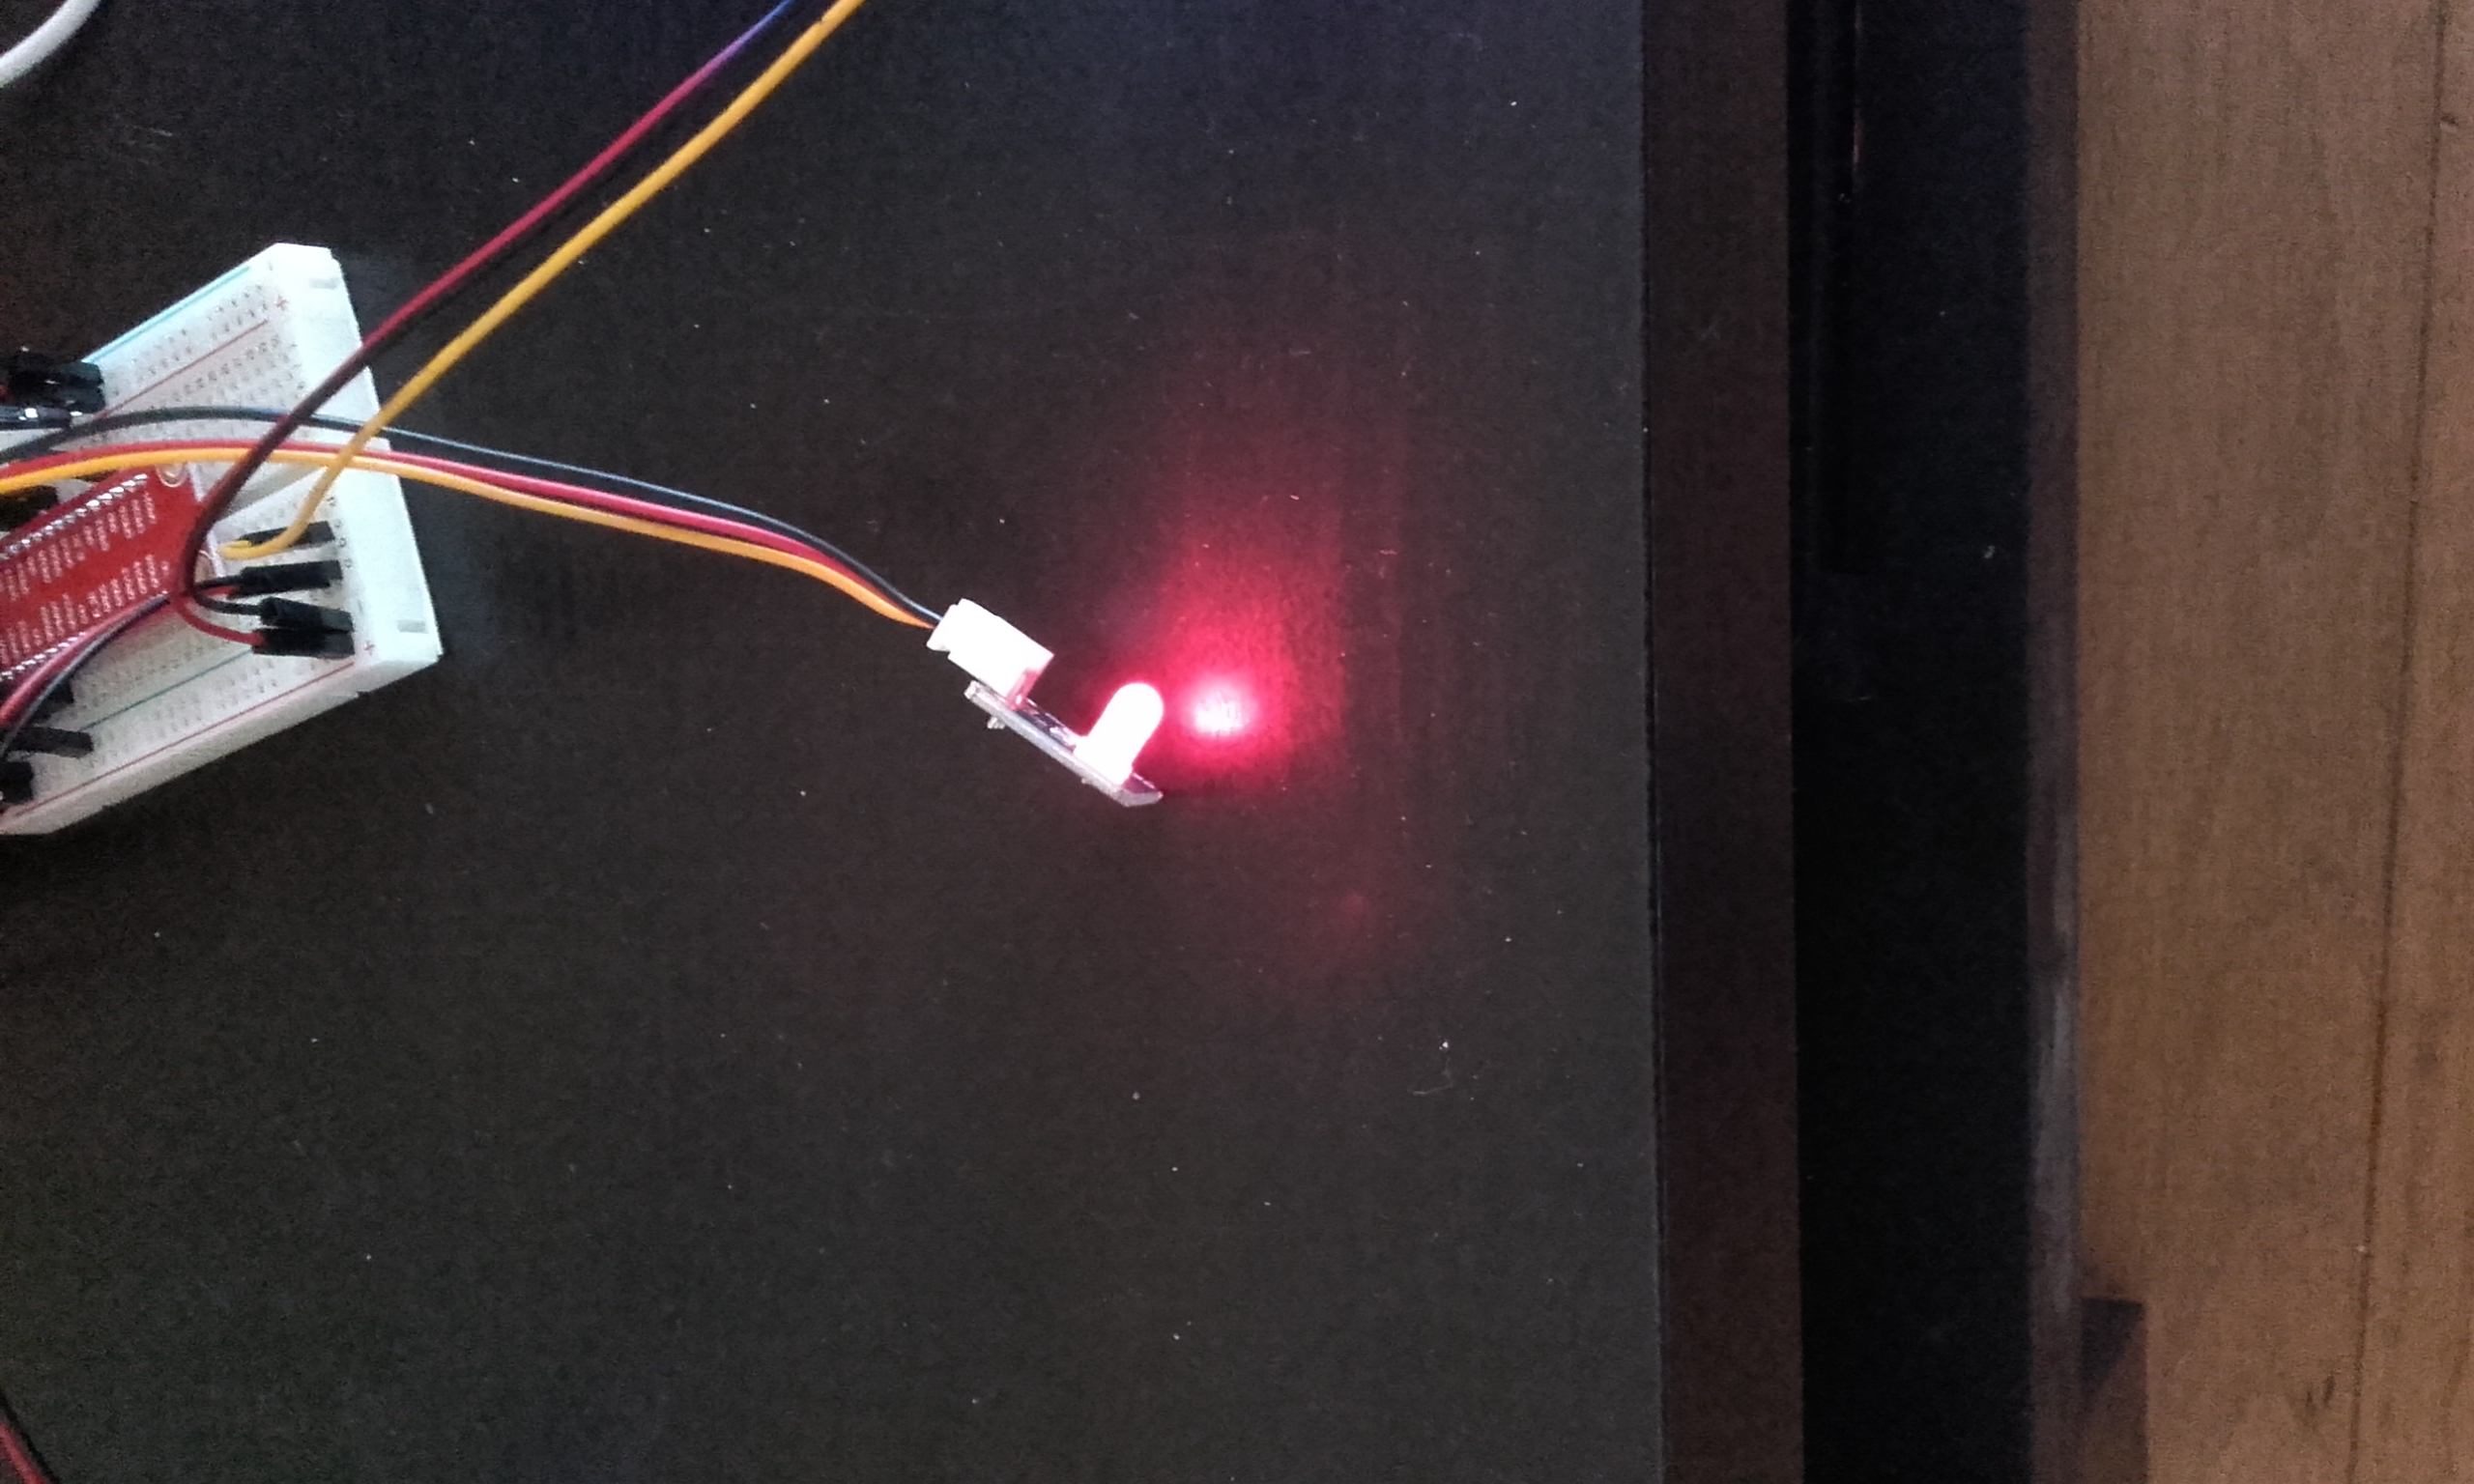
\includegraphics[width=\textwidth]{../imgs/lowTemperature.jpg}
  \caption{\label{lowTemp}Temperature lower than the reference}
\end{figure}

\begin{figure}[H]
  \centering
  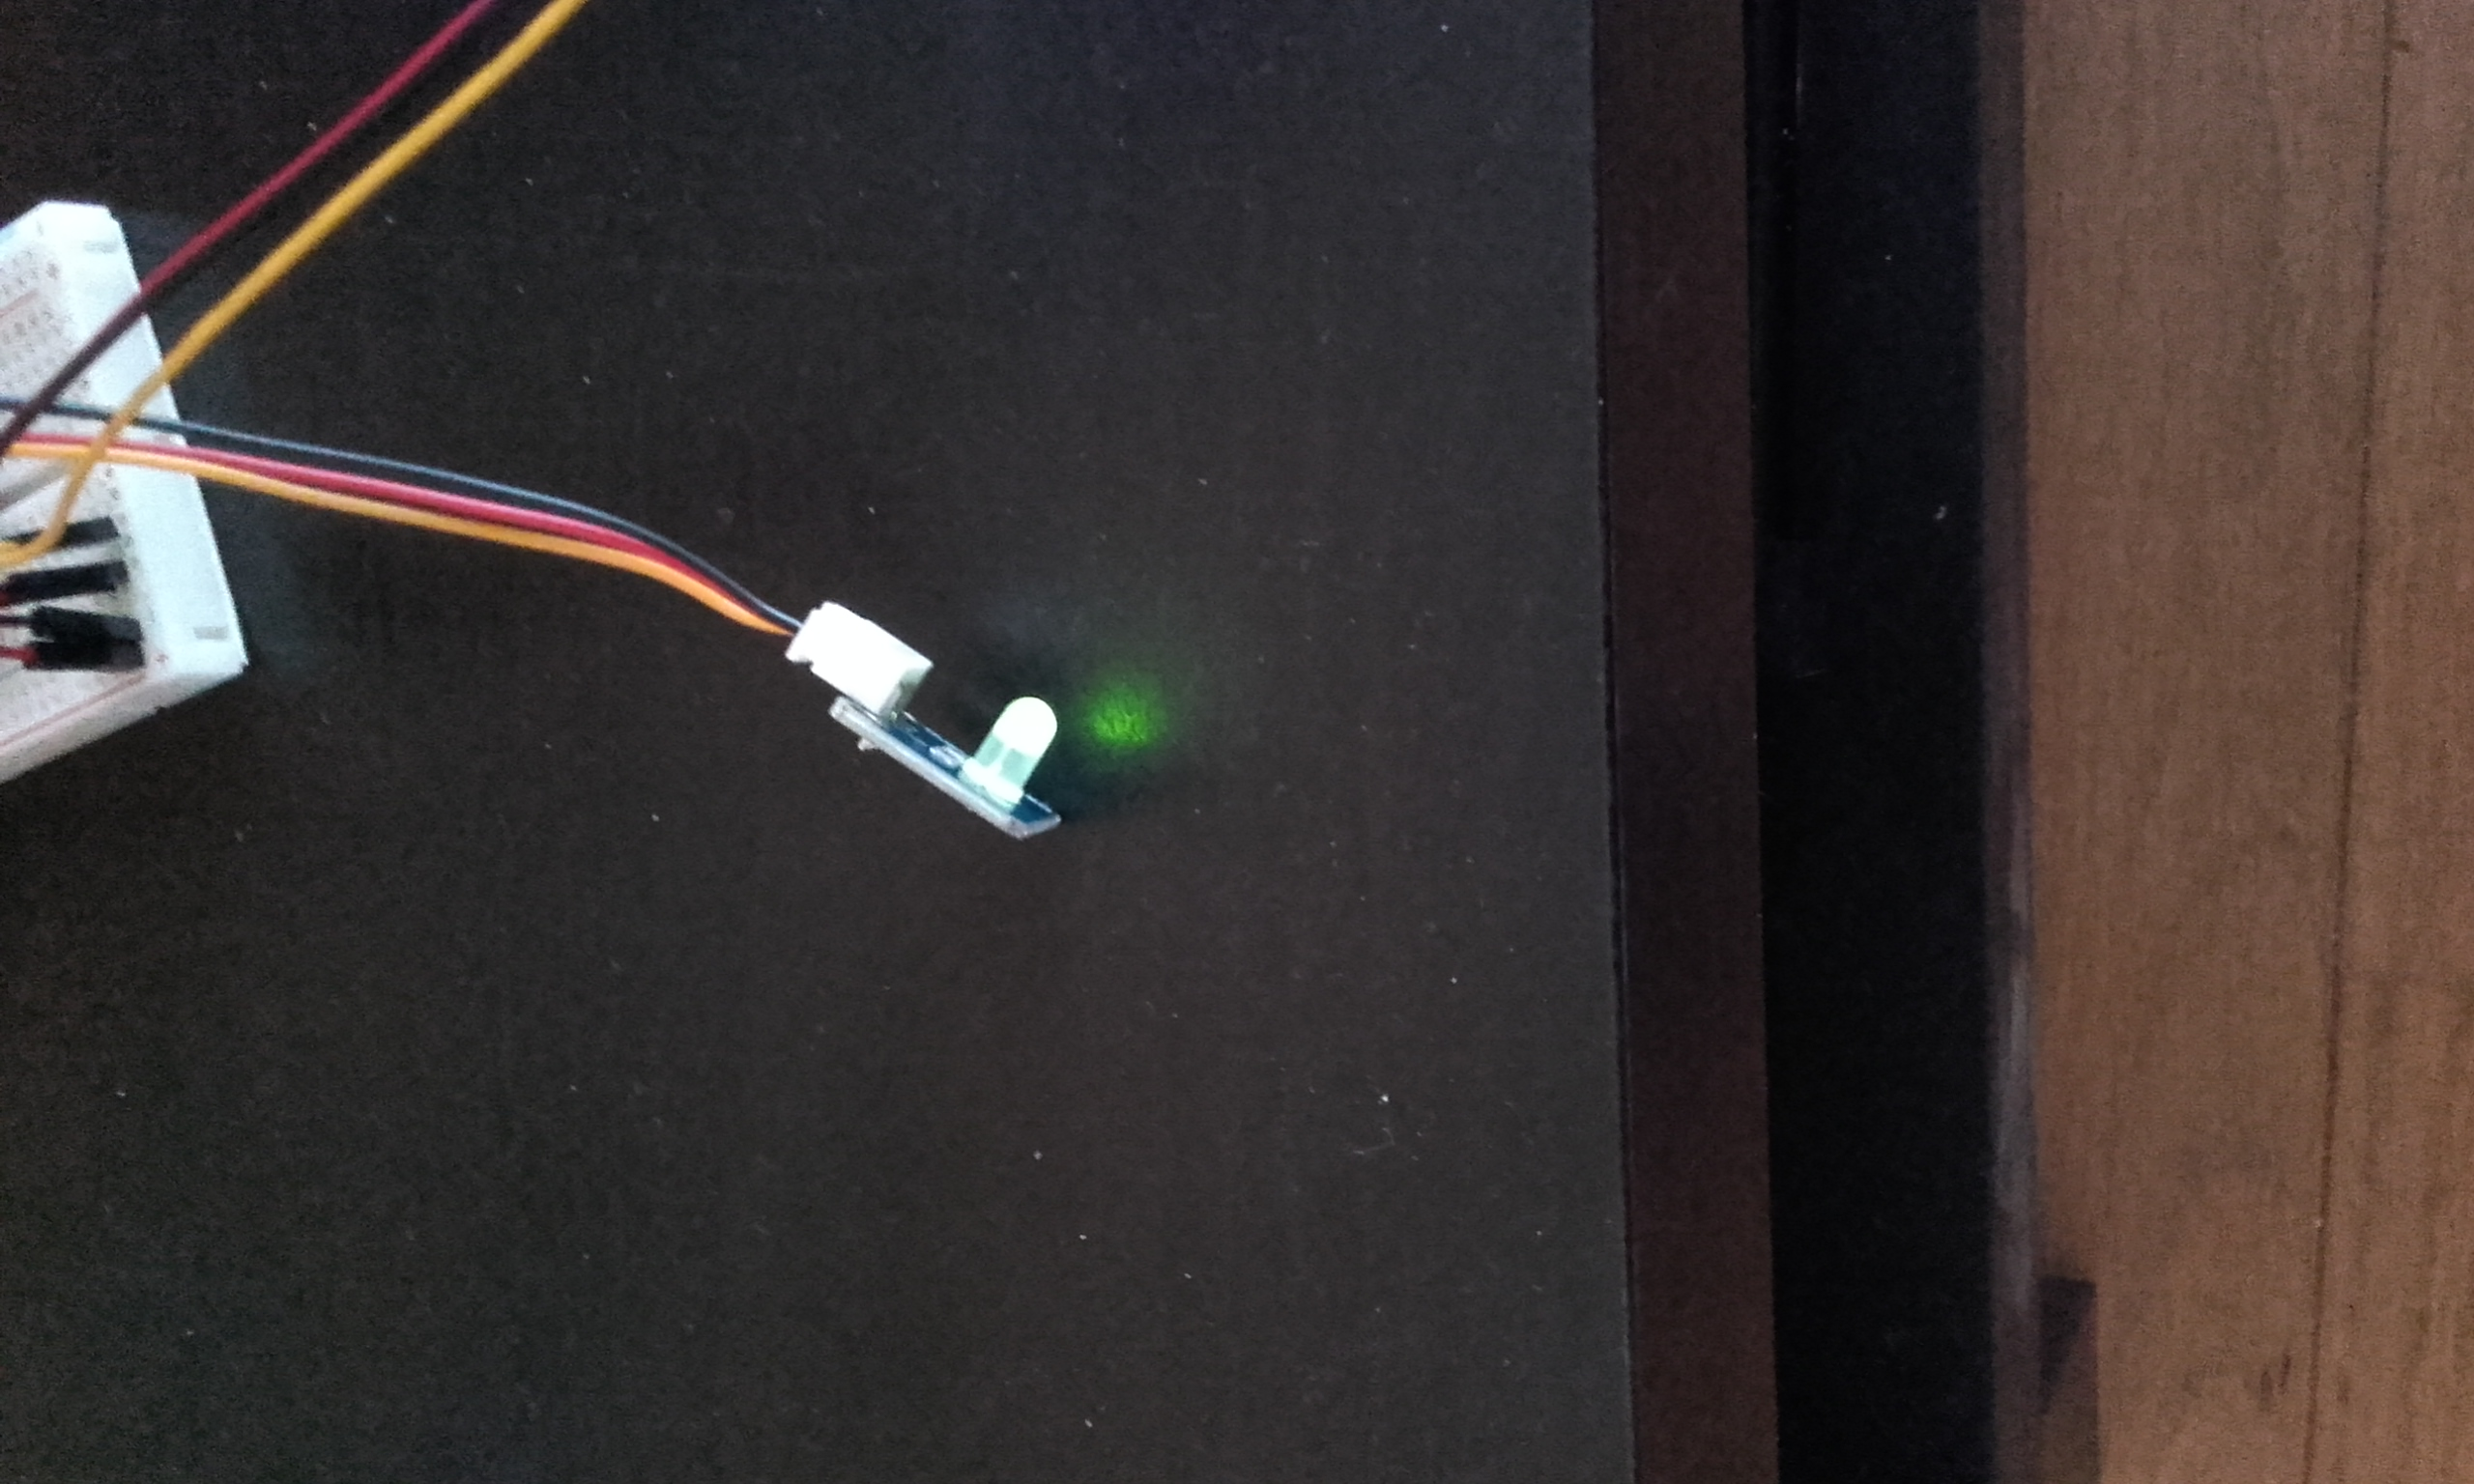
\includegraphics[width=\textwidth]{../imgs/highTemperature.jpg}
  \caption{\label{highTemp}Temperature higher than the reference}
\end{figure}

\begin{figure}[H]
  \centering
  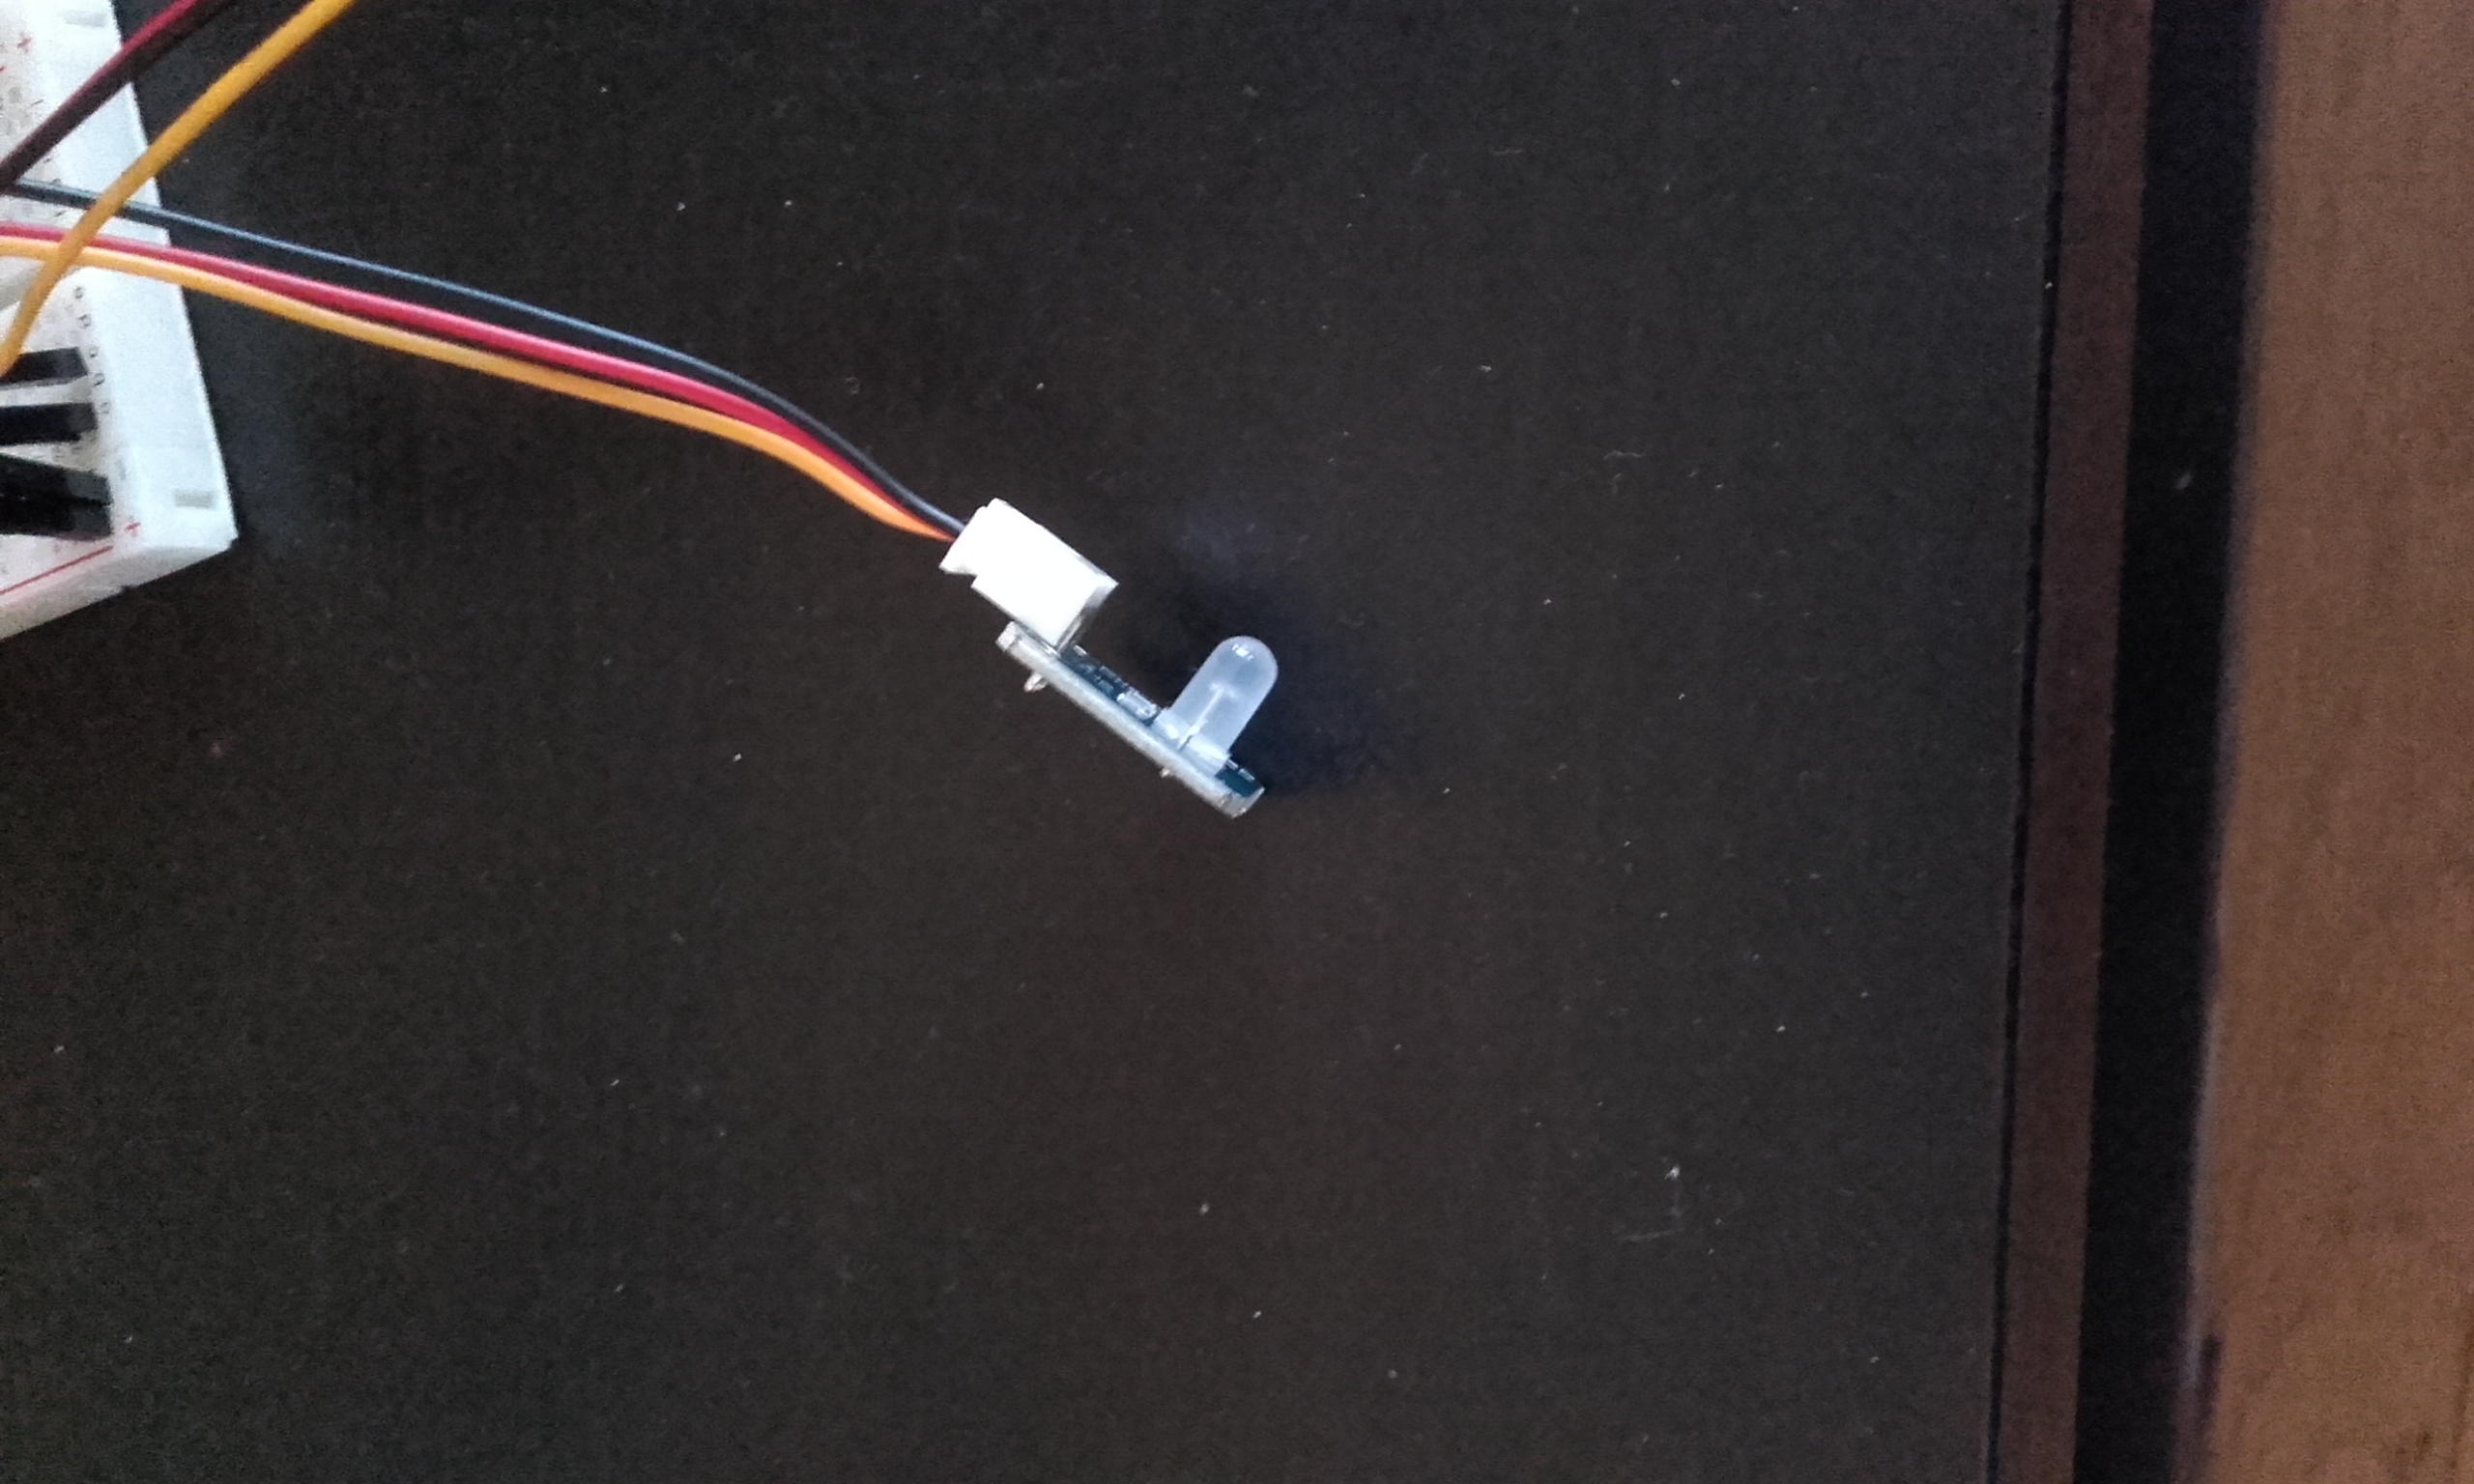
\includegraphics[width=\textwidth]{../imgs/goodTemperature.jpg}
  \caption{\label{goodTemp}Temperature equal to the reference}
\end{figure}

\subsection{Lumen management}

A button in the house (on the raspberry) can turn on or turn off the lights.

If lights are turned on, the server fixes the light power according to the lumen sensor data.
Max and min limits are hardcoded for the lumen sensor data values (variable resistance of the sensor).
\begin{itemize}
\item If the lumen sensor data value is higher than the max limit, the lights are turned off.
\item If the lumen sensor data value is lower than the min limit, the lights are turn on at maximum power.
\item If the lumen sensor data value is between the limits, the lights are turn on at power linearly depending of the value.
\end{itemize}

The raspberry which control the lights create a smooth transition between the previous light power and the new ordered by the server.

\begin{figure}[H]
  \centering
  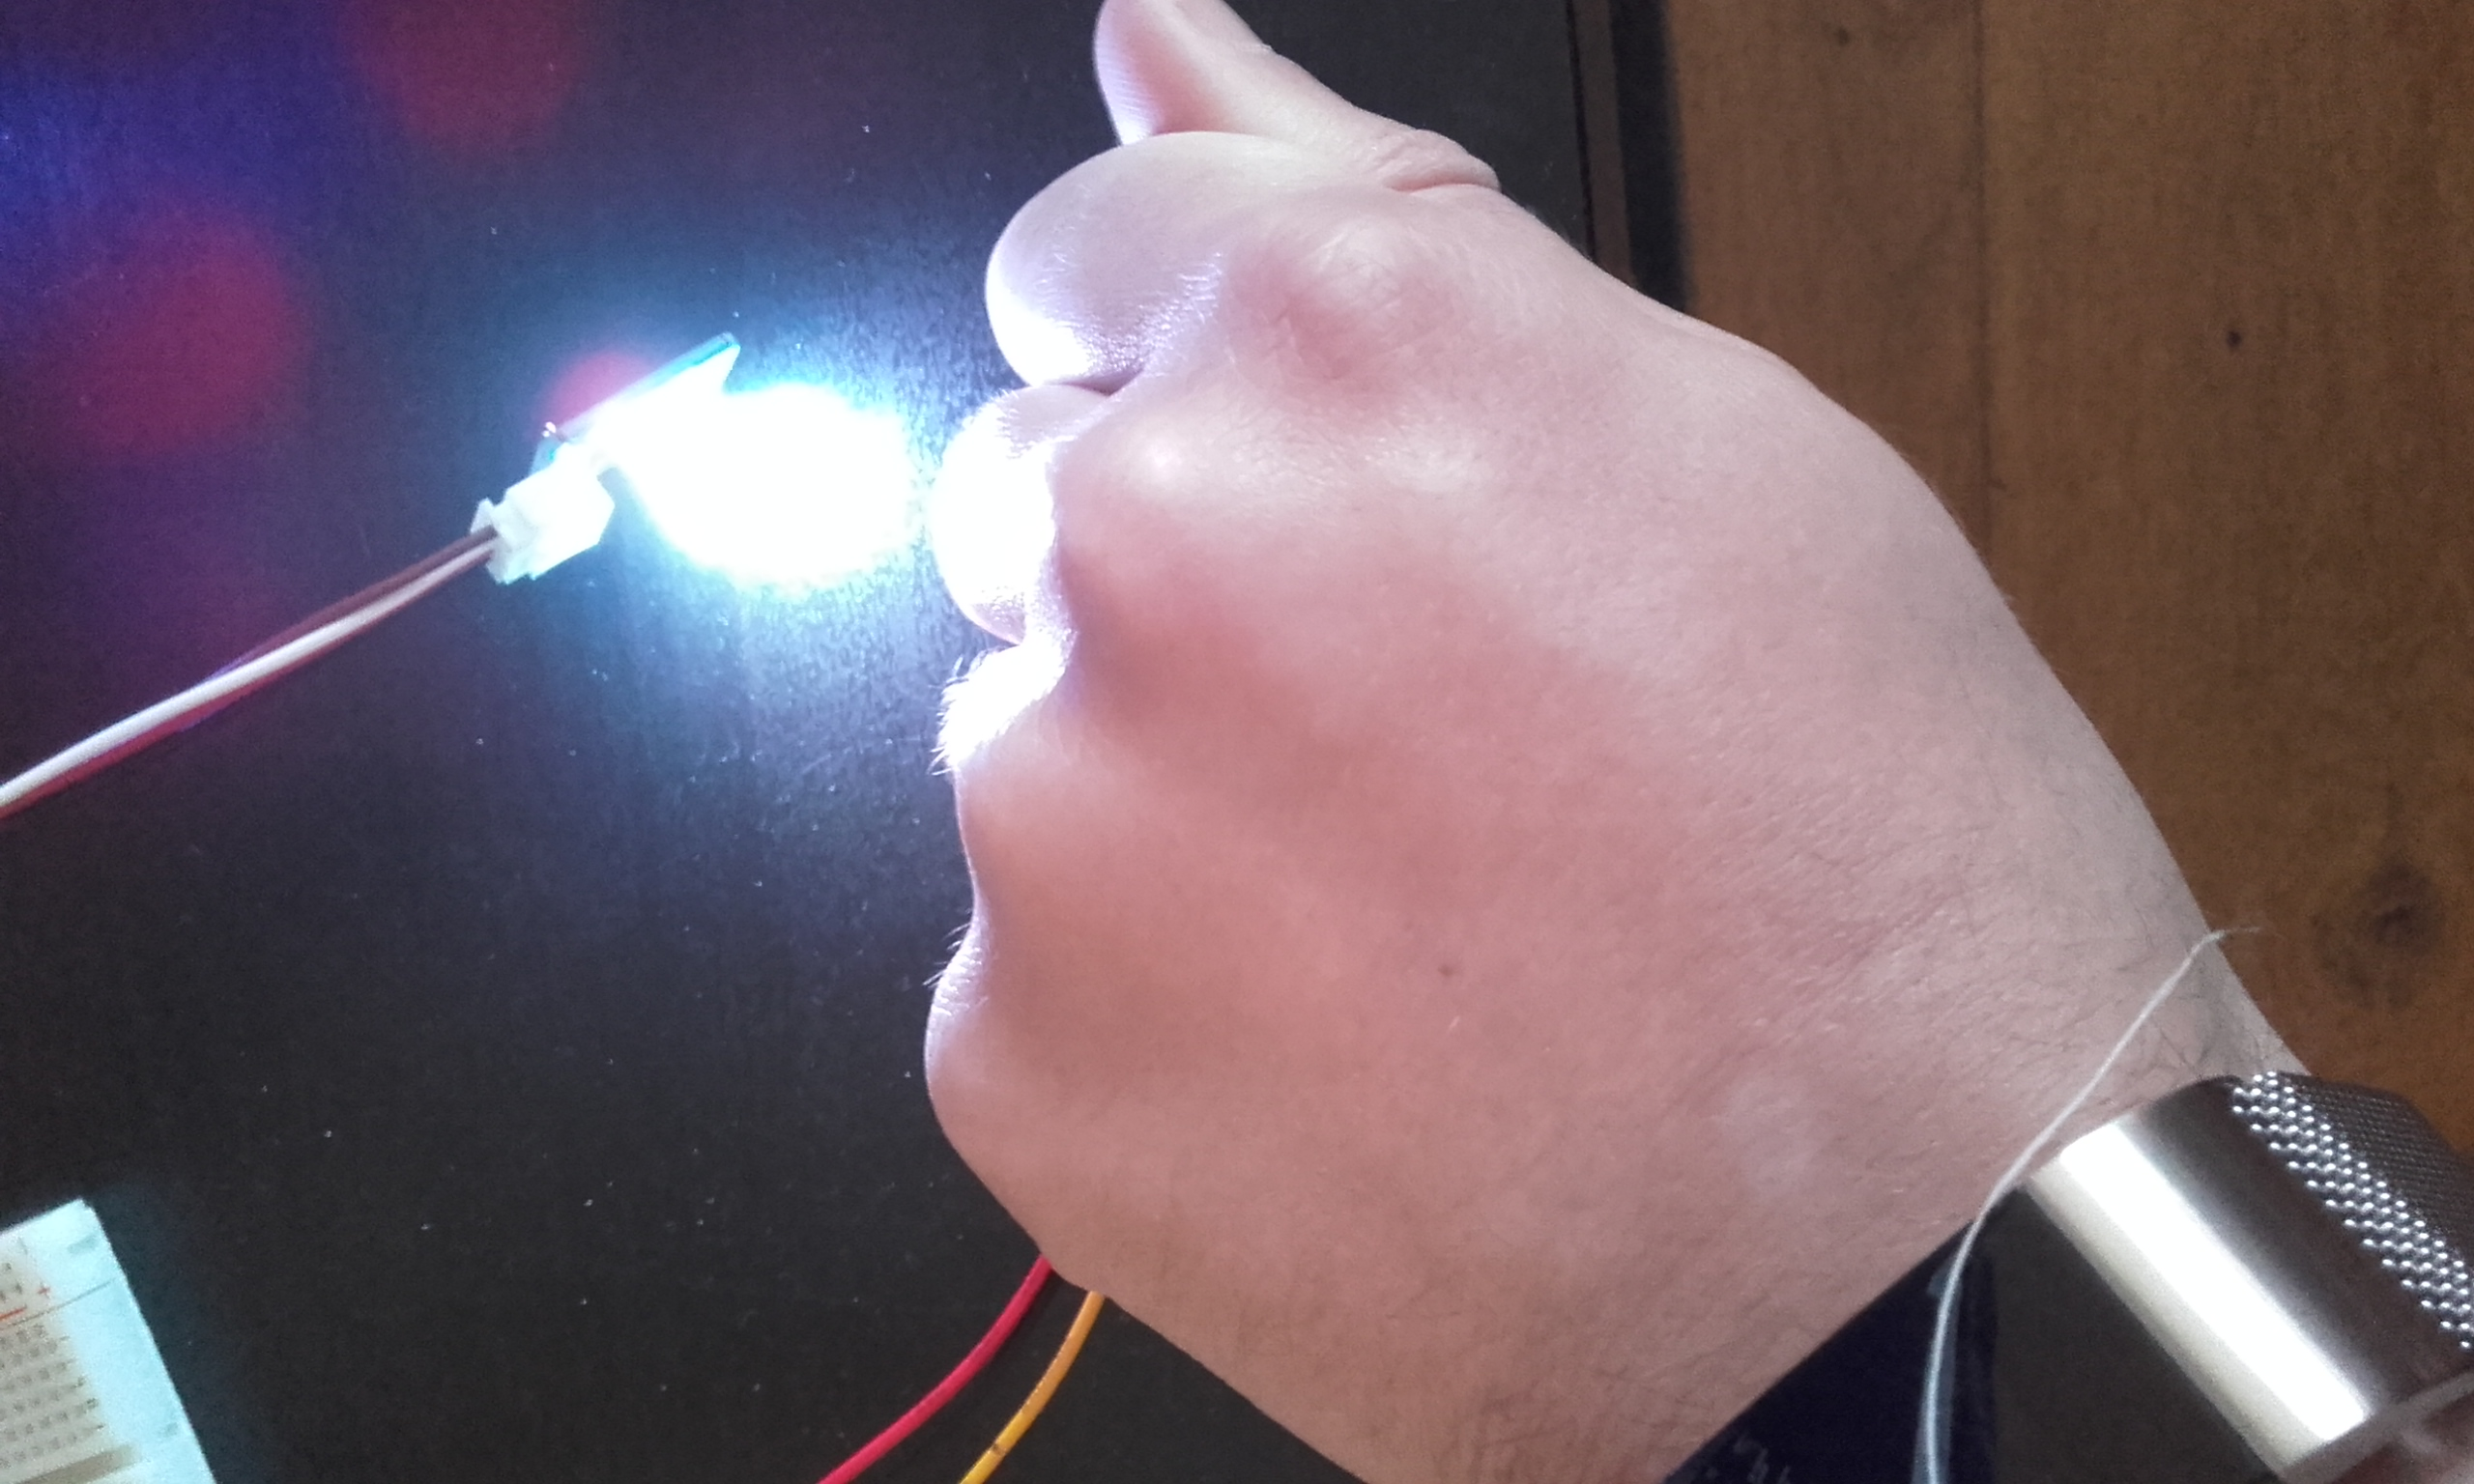
\includegraphics[width=\textwidth]{../imgs/littleBrightness2.jpg}
  \caption{\label{littleBrightness}Little brightness (lumen sensor in the closed hand)}
\end{figure}

\begin{figure}[H]
  \centering
  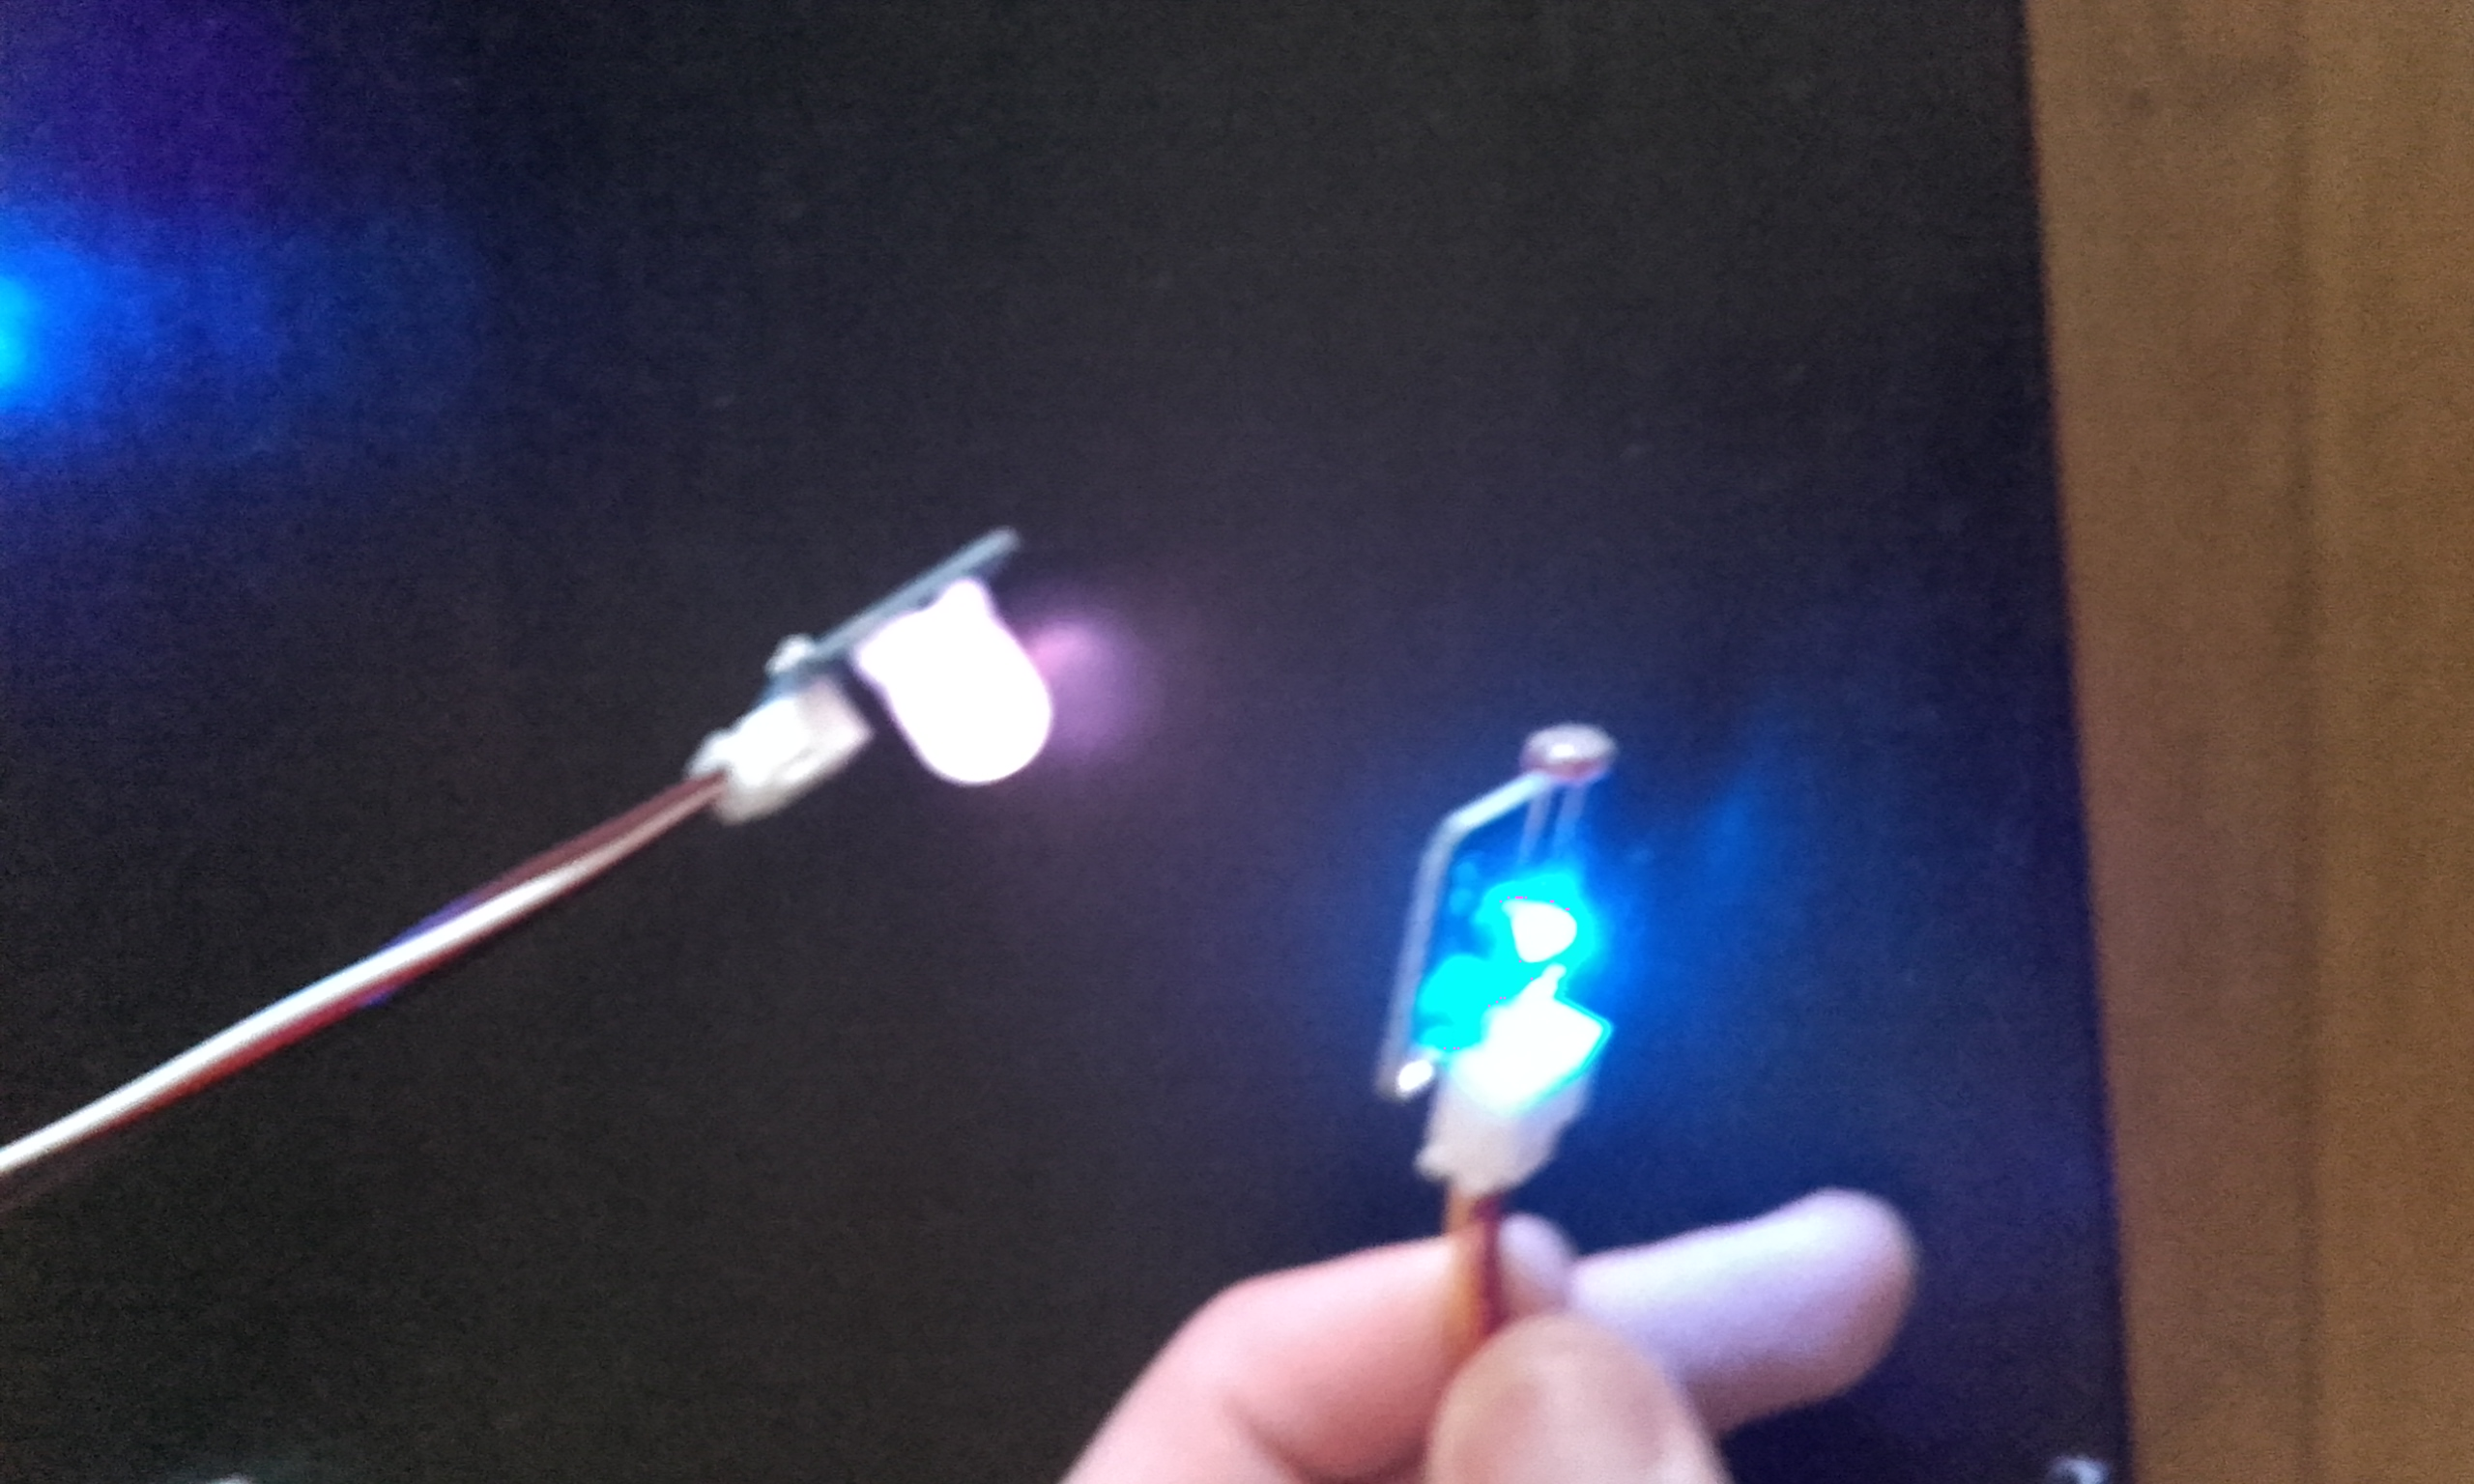
\includegraphics[width=\textwidth]{../imgs/lotOfBrightness2.jpg}
  \caption{\label{lotOfBrightness}A lot of brightness (lumen sensor facing to the window)}
\end{figure}


\section{Architecture}

\subsection{Hardware}

All sensors and actuators are fixed on the raspberry board.

\begin{figure}[H]
  \centering
  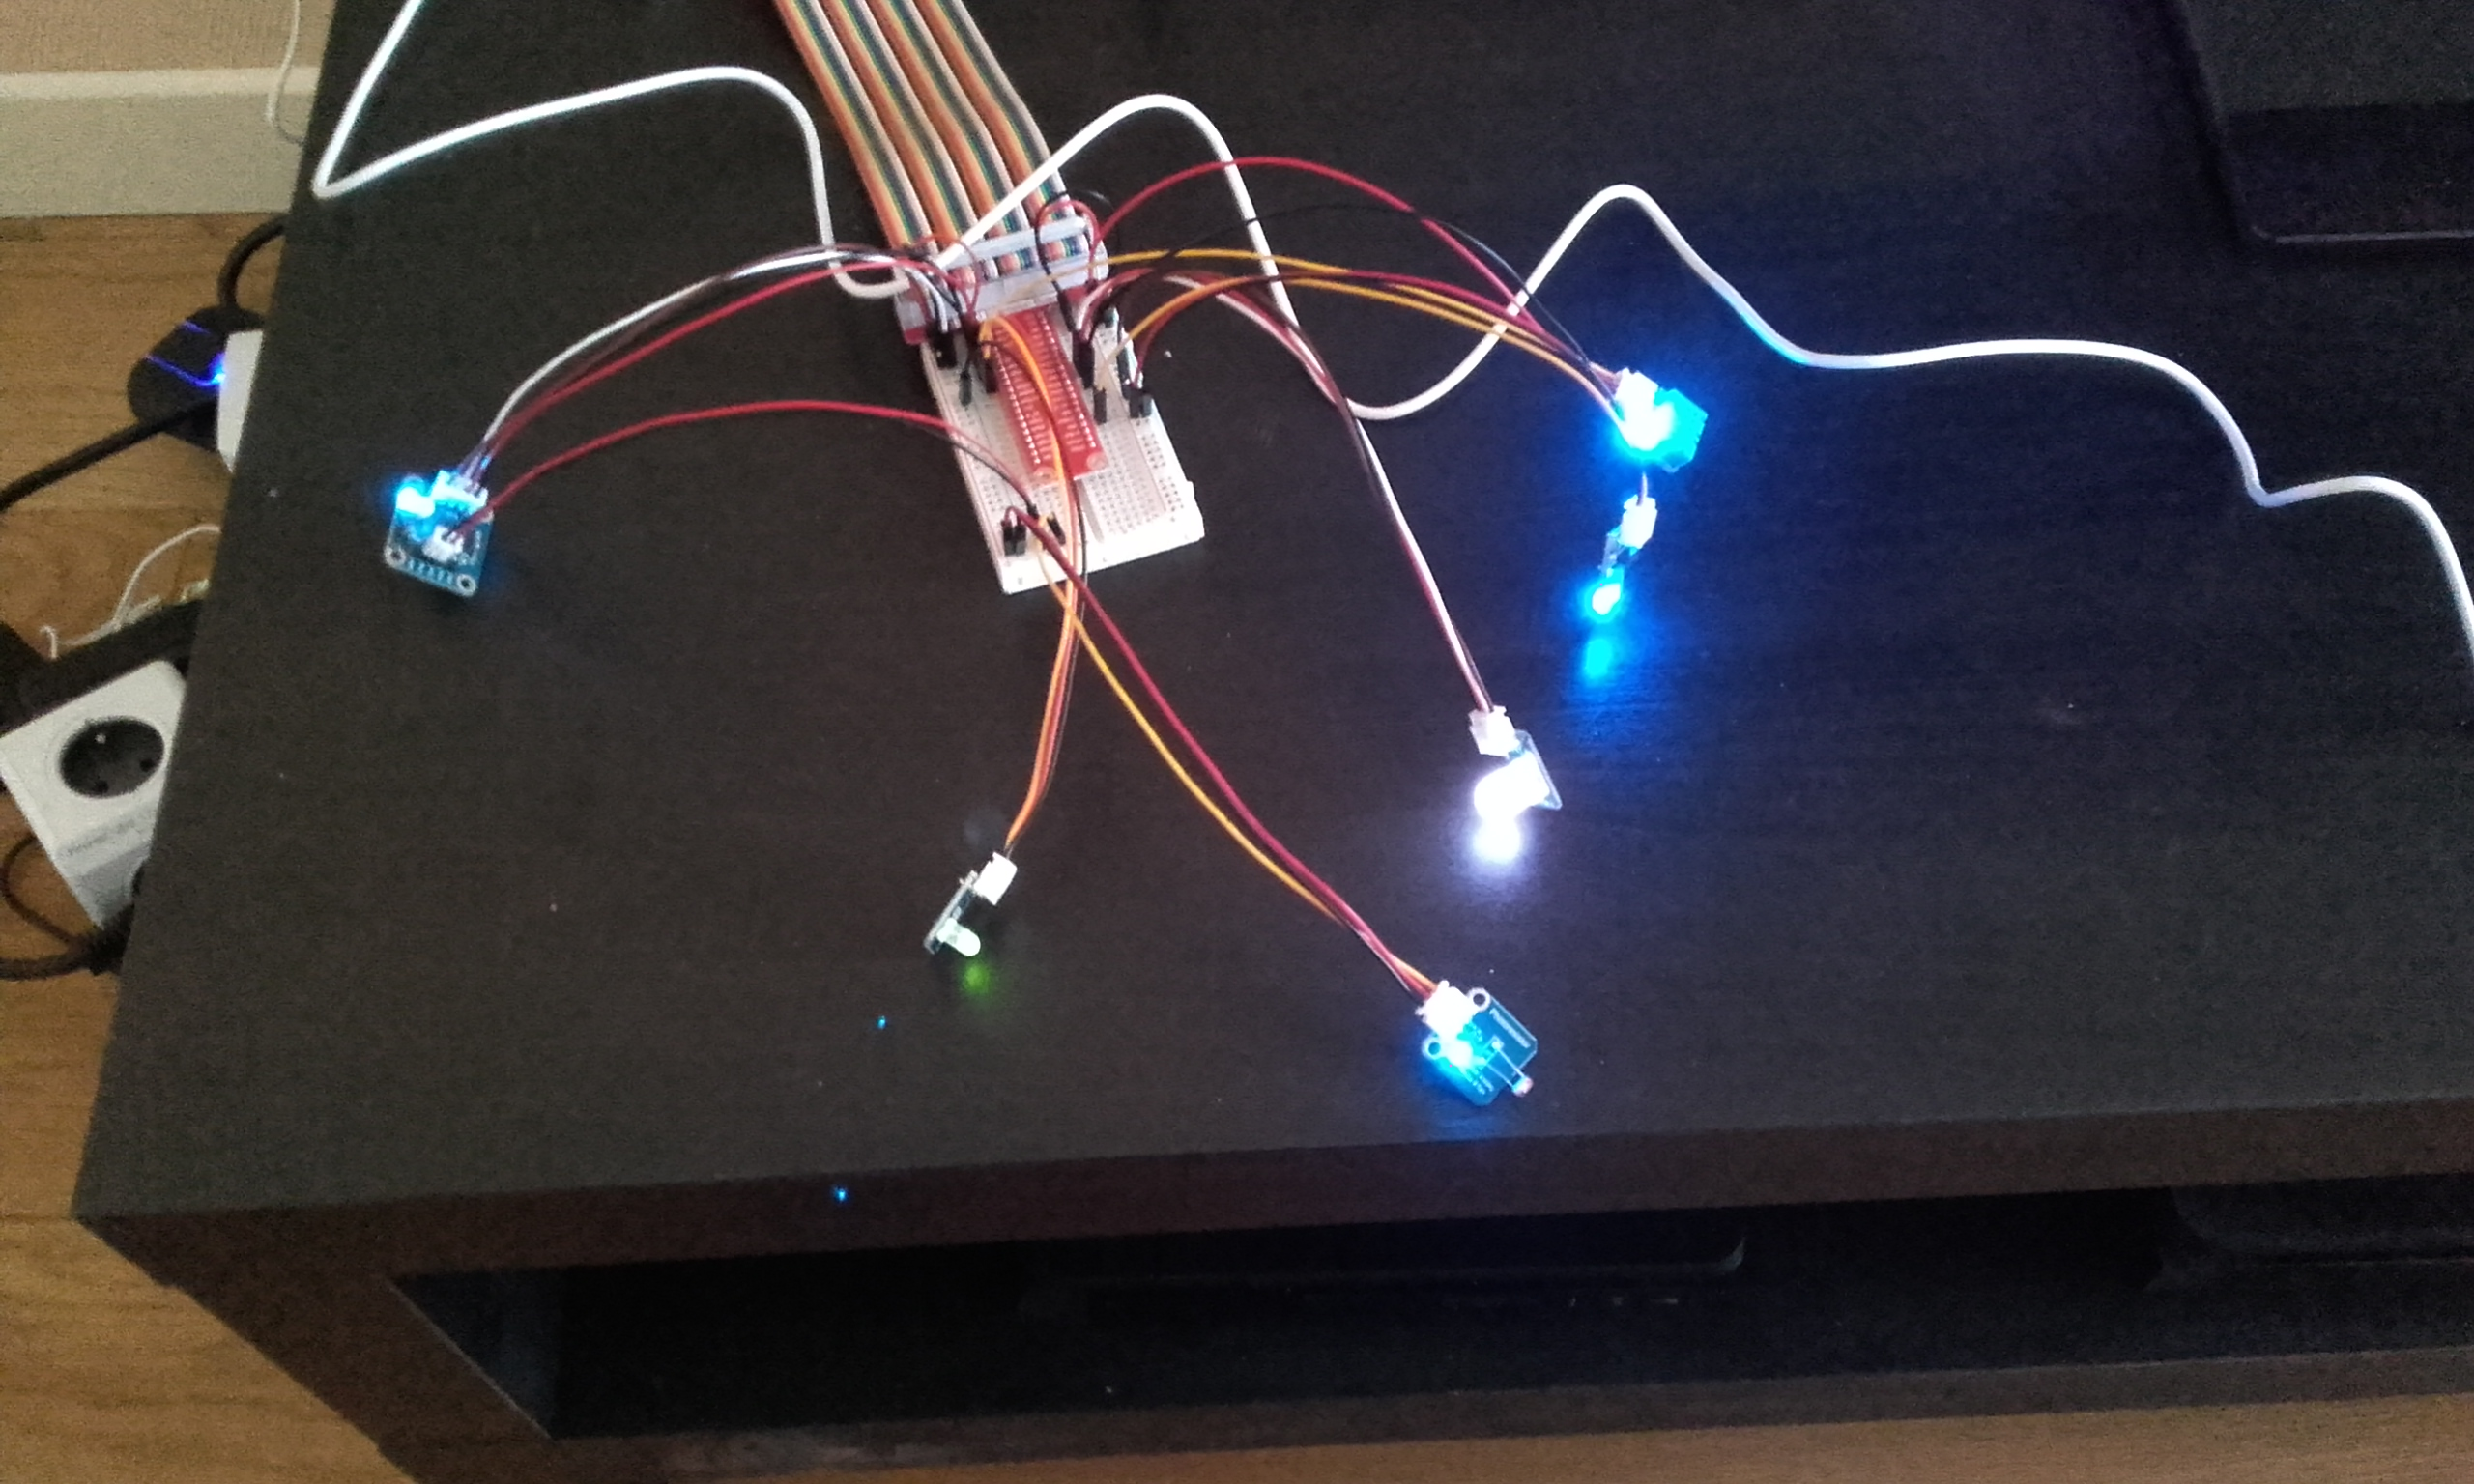
\includegraphics[width=\textwidth]{../imgs/entireSystem.jpg}
  \caption{\label{entireSystem}The entire system}
\end{figure}

\subsubsection{Assembly}
PCF8591 and Photoresistor
\begin{table}[H]
  \centering
\begin{tabular}{r c l}
  & PCF8591 & (remove the jumper)\\
  \hline
  VCC &->& 3.3V \\
  GND &->& GND \\
  SCL &->& SCL \\
  SDA &->& SDA \\
  \\
  & Photoresistor & \\
  \hline
  VCC &->& 3.3V \\
  GND &->& GND \\
  SIG &->& [PCF8591]AIN0 \\
\end{tabular}
\end{table}

Humiture Sensor

\begin{table}[H]
  \centering
\begin{tabular}{rcl}
  GND &->& GND \\
  VCC &->& 5V \\
  SIG &->& GPIO17 \\
\end{tabular}
\end{table}

Dual-Color LED

\begin{table}[H]
  \centering
\begin{tabular}{rcl}
  GND &->& GND \\
  G &->& GPIO27 \\
  R &->& GPIO22 \\
\end{tabular}
\end{table}

RGB LED

\begin{table}[H]
  \centering
\begin{tabular}{rcl}
  VCC &->& 5V \\
  R &->& GPIO23 \\
  G &->& GPIO24 \\
  B &->& GPIO25 \\
\end{tabular}
\end{table}

Button

\begin{table}[H]
  \centering
\begin{tabular}{rcl}
  V &->& 5V \\
  G &->& GND \\
  S &->& GPIO12 \\
\end{tabular}
\end{table}

\subsection{Software}

On the raspberry, a main thread is running and can display sensors information when running in a debug mode (Figure~\ref{debugMode}).
A thread is running for getting regularly sensors values (one subthread for each sensor) and store them in static variables.
A thread is running to manage the connection: one subthread to send sensors data and one other subthread to receive server commands.

On the server, one thread is running to receive raspberry sensors data, one other thread is running to send regularly commands and a third thread is running to get the reference temperature from the user.

\begin{figure}[H]
  \centering
  
\includegraphics[max width=\textwidth]{../imgs/debugMode.png}
  \caption{\label{debugMode}Debug mode running on the raspberry}
\end{figure}

\begin{figure}[H]
  \centering
  
\includegraphics[max width=\textwidth]{../imgs/debugLightsOff.png}
  \caption{\label{debugOff}Debug mode running on the raspberry with lights off notification (button pressed)}
\end{figure}


\begin{figure}[H]
  \centering
  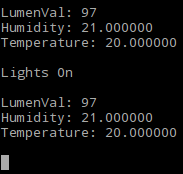
\includegraphics[max width=\textwidth]{../imgs/debugLightsOn.png}
  \caption{\label{debugOn}Debug mode running on the raspberry with lights on notification (button pressed)}
\end{figure}

\begin{figure}[H]
  \centering
  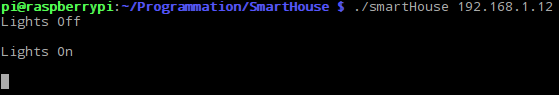
\includegraphics[max width=\textwidth]{../imgs/normalMode.png}
  \caption{\label{normalMode}Normal mode running on the raspberry with lights notifications}
\end{figure}

\end{document}
